\documentclass{standalone}
\usepackage{tikz}
\usetikzlibrary{patterns, positioning}
\usepackage[sfdefault]{ClearSans} %% option 'sfdefault' activates Clear Sans as the default text font
\usepackage[T1]{fontenc}

\begin{document}
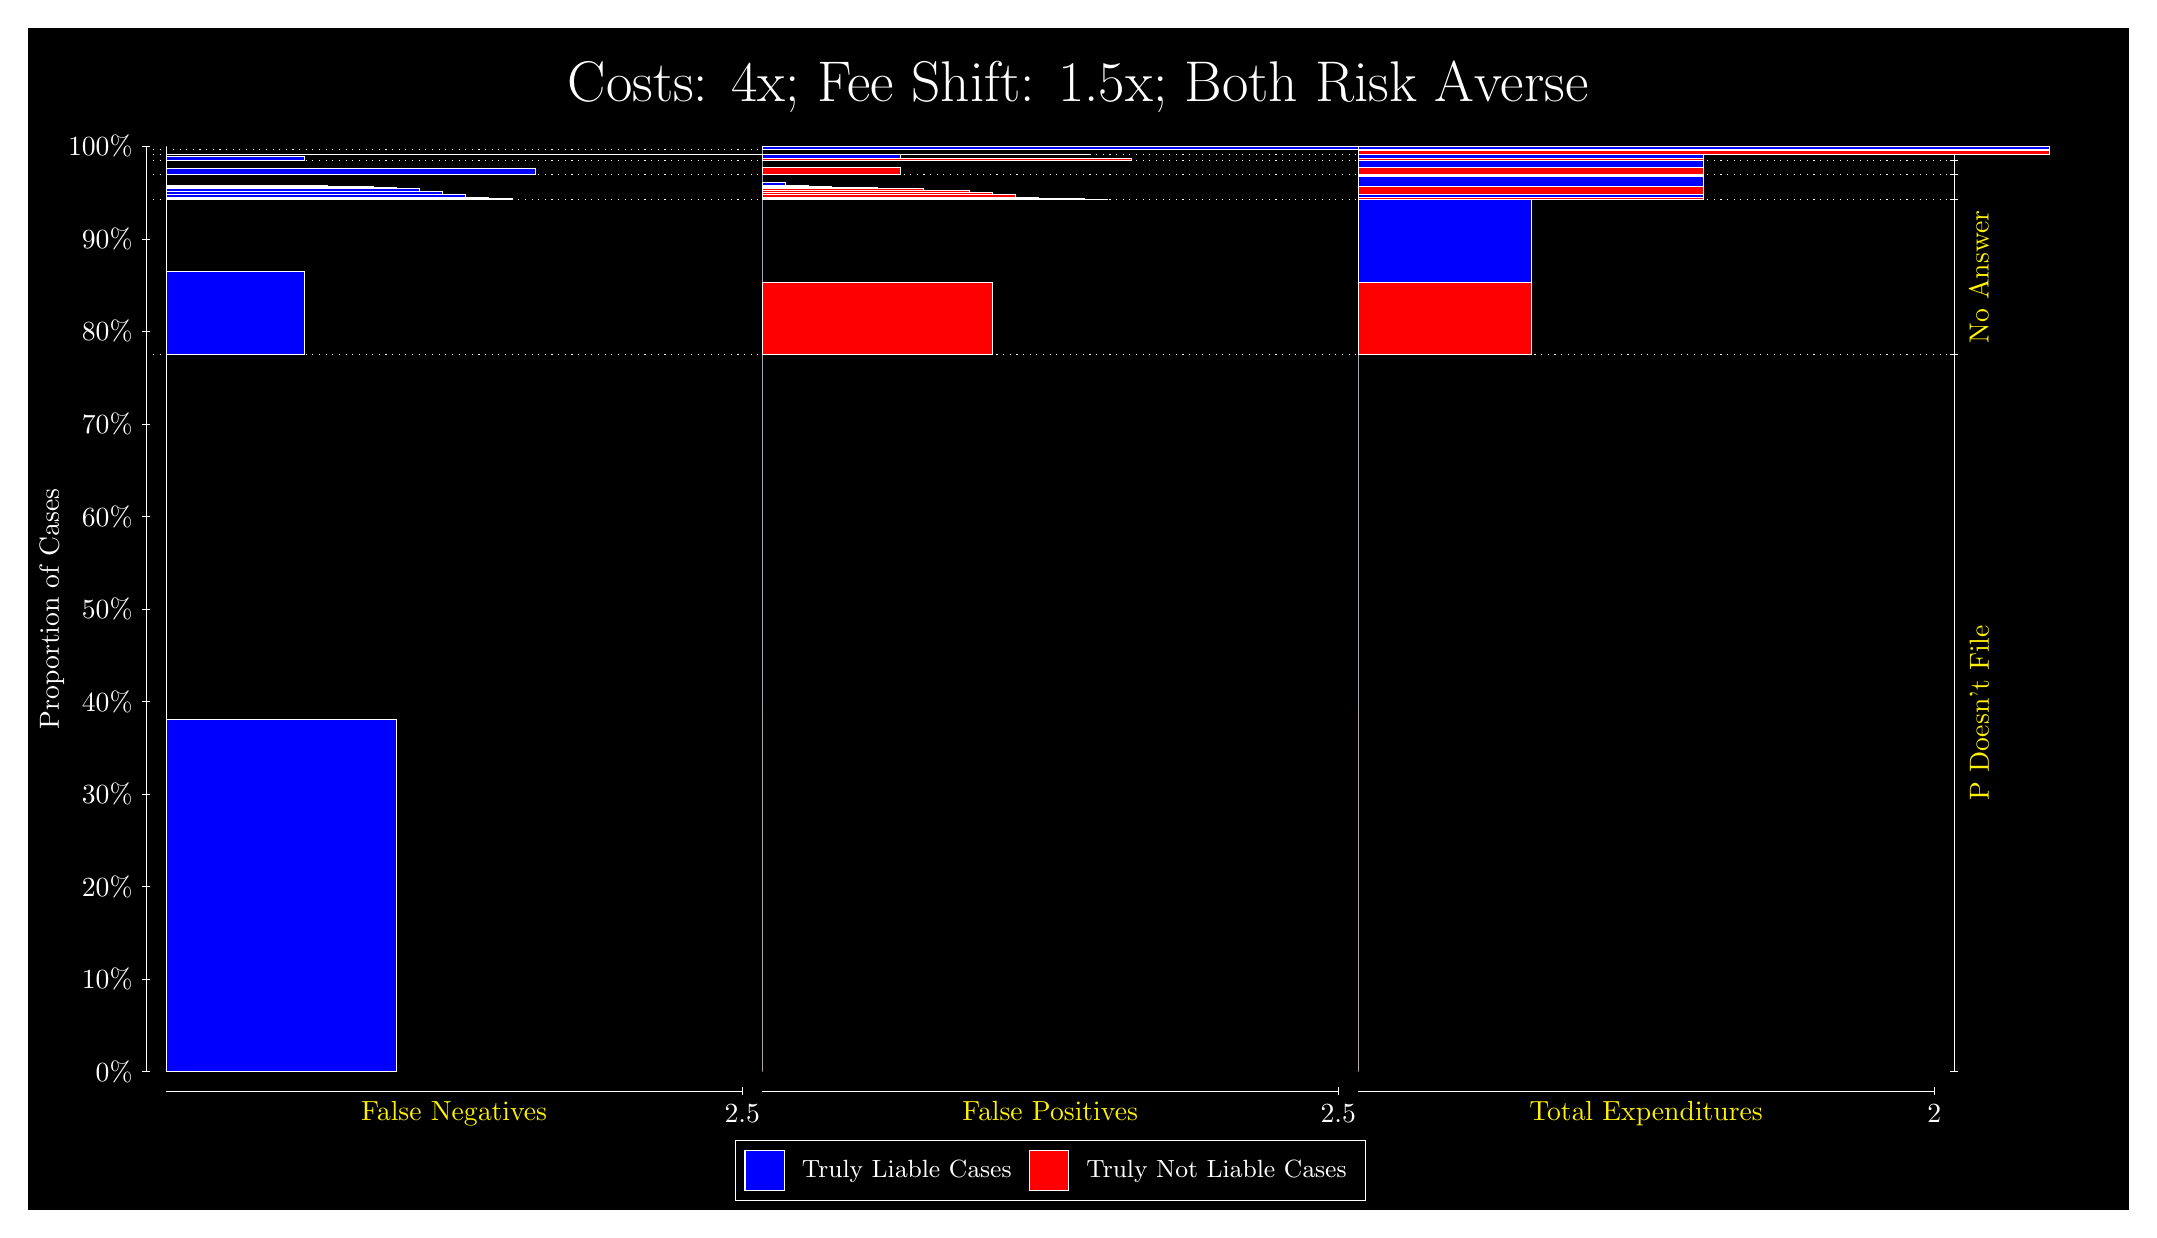
\begin{tikzpicture}
\draw[fill=black] (0,0) rectangle (26.667,15);
\draw[text=white] (0,13.5) rectangle (26.667,15) node[midway] {\huge Costs: 4x; Fee Shift: 1.5x; Both Risk Averse};
\draw[white, very thin] (1.5,1.75) -- (1.5,13.5);
\node[rotate=90, text=white, anchor=center] at (0.3, 7.625) {Proportion of Cases};
\draw[white, very thin] (1.45,1.75) -- (1.55,1.75);
\node[text=white, anchor=east] at (1.45, 1.75) {0\%};
\draw[white, very thin] (1.45,2.925) -- (1.55,2.925);
\node[text=white, anchor=east] at (1.45, 2.925) {10\%};
\draw[white, very thin] (1.45,4.1) -- (1.55,4.1);
\node[text=white, anchor=east] at (1.45, 4.1) {20\%};
\draw[white, very thin] (1.45,5.275) -- (1.55,5.275);
\node[text=white, anchor=east] at (1.45, 5.275) {30\%};
\draw[white, very thin] (1.45,6.45) -- (1.55,6.45);
\node[text=white, anchor=east] at (1.45, 6.45) {40\%};
\draw[white, very thin] (1.45,7.625) -- (1.55,7.625);
\node[text=white, anchor=east] at (1.45, 7.625) {50\%};
\draw[white, very thin] (1.45,8.8) -- (1.55,8.8);
\node[text=white, anchor=east] at (1.45, 8.8) {60\%};
\draw[white, very thin] (1.45,9.975) -- (1.55,9.975);
\node[text=white, anchor=east] at (1.45, 9.975) {70\%};
\draw[white, very thin] (1.45,11.15) -- (1.55,11.15);
\node[text=white, anchor=east] at (1.45, 11.15) {80\%};
\draw[white, very thin] (1.45,12.325) -- (1.55,12.325);
\node[text=white, anchor=east] at (1.45, 12.325) {90\%};
\draw[white, very thin] (1.45,13.5) -- (1.55,13.5);
\node[text=white, anchor=east] at (1.45, 13.5) {100\%};

\draw[white, very thin] (24.457,1.75) -- (24.457,13.5);
\draw[white, very thin] (24.407,1.75) -- (24.507,1.75);
\node[anchor=west] at (24.407, 1.75) {};
\draw[white, very thin] (24.407,10.855) -- (24.507,10.855);
\node[anchor=west] at (24.407, 10.855) {};
\draw[white, very thin] (24.407,12.827) -- (24.507,12.827);
\node[anchor=west] at (24.407, 12.827) {};
\draw[white, very thin] (24.407,13.145) -- (24.507,13.145);
\node[anchor=west] at (24.407, 13.145) {};
\draw[white, very thin] (24.407,13.319) -- (24.507,13.319);
\node[anchor=west] at (24.407, 13.319) {};
\draw[white, very thin] (24.407,13.398) -- (24.507,13.398);
\node[anchor=west] at (24.407, 13.398) {};
\draw[white, very thin] (24.407,13.457) -- (24.507,13.457);
\node[anchor=west] at (24.407, 13.457) {};
\draw[white, very thin] (24.407,13.5) -- (24.507,13.5);
\node[anchor=west] at (24.407, 13.5) {};

\draw[white, very thin, fill=blue] (1.75,1.75) rectangle (4.6775,6.224);
\draw[white, very thin, fill=red] (1.75,6.224) rectangle (1.75,10.855);
\draw[white, very thin, fill=blue] (1.75,10.855) rectangle (3.5065,11.911);
\draw[white, very thin, fill=red] (1.75,11.911) rectangle (1.75,12.827);
\draw[white, very thin, fill=blue] (1.75,12.827) rectangle (6.1413,12.844);
\draw[white, very thin, fill=blue] (1.75,12.844) rectangle (5.8486,12.854);
\draw[white, very thin, fill=blue] (1.75,12.854) rectangle (5.5558,12.891);
\draw[white, very thin, fill=blue] (1.75,12.891) rectangle (5.2631,12.933);
\draw[white, very thin, fill=blue] (1.75,12.933) rectangle (4.9703,12.971);
\draw[white, very thin, fill=blue] (1.75,12.971) rectangle (4.6775,12.984);
\draw[white, very thin, fill=blue] (1.75,12.984) rectangle (4.3848,12.993);
\draw[white, very thin, fill=blue] (1.75,12.993) rectangle (4.092,12.998);
\draw[white, very thin, fill=blue] (1.75,12.998) rectangle (3.7993,13.002);
\draw[white, very thin, fill=red] (1.75,13.002) rectangle (1.75,13.145);
\draw[white, very thin, fill=blue] (1.75,13.145) rectangle (6.4341,13.224);
\draw[white, very thin, fill=red] (1.75,13.224) rectangle (1.75,13.319);
\draw[white, very thin, fill=blue] (1.75,13.319) rectangle (3.5065,13.368);
\draw[white, very thin, fill=red] (1.75,13.368) rectangle (1.75,13.398);
\draw[white, very thin, fill=blue] (1.75,13.398) rectangle (13.46,13.401);
\draw[white, very thin, fill=red] (1.75,13.401) rectangle (1.75,13.457);
\draw[white, very thin, fill=red] (1.75,13.457) rectangle (1.75,13.461);
\draw[white, very thin, fill=blue] (1.75,13.461) rectangle (1.75,13.5);
\draw[white, very thin, fill=red] (9.3189,1.75) rectangle (9.3189,6.3814);
\draw[white, very thin, fill=blue] (9.3189,6.3814) rectangle (9.3189,10.855);
\draw[white, very thin, fill=red] (9.3189,10.855) rectangle (12.246,11.771);
\draw[white, very thin, fill=blue] (9.3189,11.771) rectangle (9.3189,12.827);
\draw[white, very thin, fill=red] (9.3189,12.827) rectangle (13.71,12.831);
\draw[white, very thin, fill=red] (9.3189,12.831) rectangle (13.417,12.835);
\draw[white, very thin, fill=red] (9.3189,12.835) rectangle (13.125,12.846);
\draw[white, very thin, fill=red] (9.3189,12.846) rectangle (12.832,12.859);
\draw[white, very thin, fill=red] (9.3189,12.859) rectangle (12.539,12.888);
\draw[white, very thin, fill=red] (9.3189,12.888) rectangle (12.246,12.914);
\draw[white, very thin, fill=red] (9.3189,12.914) rectangle (11.954,12.938);
\draw[white, very thin, fill=red] (9.3189,12.938) rectangle (11.661,12.944);
\draw[white, very thin, fill=red] (9.3189,12.944) rectangle (11.368,12.97);
\draw[white, very thin, fill=blue] (9.3189,12.97) rectangle (10.783,12.974);
\draw[white, very thin, fill=blue] (9.3189,12.974) rectangle (10.49,12.978);
\draw[white, very thin, fill=blue] (9.3189,12.978) rectangle (10.197,12.988);
\draw[white, very thin, fill=blue] (9.3189,12.988) rectangle (9.9044,13.001);
\draw[white, very thin, fill=blue] (9.3189,13.001) rectangle (9.6116,13.039);
\draw[white, very thin, fill=blue] (9.3189,13.039) rectangle (9.3189,13.145);
\draw[white, very thin, fill=red] (9.3189,13.145) rectangle (11.075,13.24);
\draw[white, very thin, fill=blue] (9.3189,13.24) rectangle (9.3189,13.319);
\draw[white, very thin, fill=red] (9.3189,13.319) rectangle (14.003,13.349);
\draw[white, very thin, fill=blue] (9.3189,13.349) rectangle (11.075,13.398);
\draw[white, very thin, fill=red] (9.3189,13.398) rectangle (9.3189,13.454);
\draw[white, very thin, fill=blue] (9.3189,13.454) rectangle (9.3189,13.457);
\draw[white, very thin, fill=red] (9.3189,13.457) rectangle (21.029,13.461);
\draw[white, very thin, fill=blue] (9.3189,13.461) rectangle (18.102,13.5);
\draw[white, very thin, fill=red] (16.888,1.75) rectangle (16.888,6.3814);
\draw[white, very thin, fill=blue] (16.888,6.3814) rectangle (16.888,10.855);
\draw[white, very thin, fill=red] (16.888,10.855) rectangle (19.083,11.771);
\draw[white, very thin, fill=blue] (16.888,11.771) rectangle (19.083,12.827);
\draw[white, very thin, fill=red] (16.888,12.827) rectangle (21.279,12.856);
\draw[white, very thin, fill=blue] (16.888,12.856) rectangle (21.279,12.894);
\draw[white, very thin, fill=red] (16.888,12.894) rectangle (21.279,12.993);
\draw[white, very thin, fill=blue] (16.888,12.993) rectangle (21.279,13.116);
\draw[white, very thin, fill=red] (16.888,13.116) rectangle (21.279,13.131);
\draw[white, very thin, fill=blue] (16.888,13.131) rectangle (21.279,13.145);
\draw[white, very thin, fill=red] (16.888,13.145) rectangle (21.279,13.24);
\draw[white, very thin, fill=blue] (16.888,13.24) rectangle (21.279,13.319);
\draw[white, very thin, fill=red] (16.888,13.319) rectangle (21.279,13.349);
\draw[white, very thin, fill=blue] (16.888,13.349) rectangle (21.279,13.398);
\draw[white, very thin, fill=red] (16.888,13.398) rectangle (25.67,13.454);
\draw[white, very thin, fill=blue] (16.888,13.454) rectangle (25.67,13.457);
\draw[white, very thin, fill=red] (16.888,13.457) rectangle (25.67,13.461);
\draw[white, very thin, fill=blue] (16.888,13.461) rectangle (25.67,13.5);
\draw[white, dotted] (1.5,10.855) -- (24.457,10.855);
\draw[white, dotted] (1.5,12.827) -- (24.457,12.827);
\draw[white, dotted] (1.5,13.145) -- (24.457,13.145);
\draw[white, dotted] (1.5,13.319) -- (24.457,13.319);
\draw[white, dotted] (1.5,13.398) -- (24.457,13.398);
\draw[white, dotted] (1.5,13.457) -- (24.457,13.457);
\draw[white, very thin] (1.75,1.5) -- (9.0689,1.5);
\node[text=yellow, anchor=north] at (5.4094, 1.5) {False Negatives};
\draw[white, very thin] (9.0689,1.45) -- (9.0689,1.55);
\node[text=white, anchor=north] at (9.0689, 1.45) {2.5};

\draw[white, very thin] (9.3189,1.5) -- (16.638,1.5);
\node[text=yellow, anchor=north] at (12.978, 1.5) {False Positives};
\draw[white, very thin] (16.638,1.45) -- (16.638,1.55);
\node[text=white, anchor=north] at (16.638, 1.45) {2.5};

\draw[white, very thin] (16.888,1.5) -- (24.207,1.5);
\node[text=yellow, anchor=north] at (20.547, 1.5) {Total Expenditures};
\draw[white, very thin] (24.207,1.45) -- (24.207,1.55);
\node[text=white, anchor=north] at (24.207, 1.45) {2};

\node[text=yellow, centered, rotate=90] at (24.777, 6.3027) {P Doesn't File};
\node[text=yellow, centered, rotate=90] at (24.777, 11.841) {No Answer};






\draw (12.978300999999998,1.5) node[draw=none] (baseCoordinate) {};
\begin{scope}[align=center]
        \matrix[scale=0.5, draw=white, below=0.5cm of baseCoordinate, nodes={draw}, column sep=0.1cm]{
            \node[rectangle, draw, minimum width=0.5cm, minimum height=0.5cm, fill=blue] {}; &
            \node[draw=none, font=\small, text=white] (B) {Truly Liable Cases}; &
            \node[rectangle, draw, minimum width=0.5cm, minimum height=0.5cm, fill=red] {}; &
            \node[draw=none, font=\small, text=white] (B) {Truly Not Liable Cases}; \\
            };
\end{scope}

\end{tikzpicture}
\end{document}